\section{Lecture 1}
%Samuel
\subsection{Introduction}
Monte Carlo is a numerical method of measure based on random numbers. It can be used to perform a vast variety of tasks, such as computing integrals (Monte Carlo integration) or performing averages of functions on known ensembles. \\
A simple example of MC integration can be the following:
we want to compute the area of a unitary circle, in order to do that we can draw random points on its quadrature, by dividing the number of points in the circle by the total number of points in the square we get the area of the circle. \\
A typical example of MC for computing averages is the one of the Nile river. In order to compute its average depth we could use the following procedure:
\begin{itemize}
    \item Pick a point on the river
    \item Measure the depth
    \item Try a move
    \item If on the river accept
    \item Measure the depth
    \item Else reject the move
    \item Repeat
\end{itemize}
\footnote{if I reject the move I still need to count one more time the last depth.}
With this procedure the average of our function $f\left(x\right)$, the depth in the Nile case, is then given by $\frac{1}{N} \sum_{k=1}^N f \left(x_k\right)$.\\
We could have also used another procedure: setting a uniform grid over a large area that contains the river, picking random points on that grid and using those points as $x_k$. Though this would have been much less efficient because most of the points would have fallen out of the river.
\smallskip
\\
In general the two main characteristics that an MC algorithm must follow are \textbf{stationarity} and \textbf{ergodicity}.
 \subsection{How to check ergodicity}
In order to check ergodicity one should imagine starting from one single copy of the system in one particular state. If from any state i it is possible to reach any other possible state j with a finite number of steps then the algorithm is ergodic.
\subsection{How to check stationarity}
Imagine having a large number of copies of the system distributed with $p\left(x\right)$, where $p\left(x\right)$ is the probability of being in state x. If, after applying the algorithm to all the copies of the system, we still have an ensemble of systems distributed with $p\left(x\right)$, then the algorithm is stationary for this distribution.
\smallskip
\\
In the following example we will present an algorithm that is stationary, but not ergodic.
Let us suppose we have an ensemble of systems distributed with a pdf which is a 2-D Gaussian centred at $\left(x,y\right)=\left(0,0\right)$ in some frame of reference. Consider an algorithm that at every step rotates the points of a certain angle. Such an algorithm will surely be stationary, in fact the distribution of the ensemble of systems after any iteration will always be the same. Ergodicity though is broken, in fact if we consider now the evolution of one single system (a point in the 2-D plane in our case), it can only have access to a circumference and not to the whole plane.
\smallskip
\\
How can such an algorithm be made ergodic?
\smallskip
\\
We could for example choose randomly if to move angle or radius, then move randomly angle or radius.
\subsection{Transition matrices}
In order to make the previous definitions more quantitative it is useful to introduce the formalism of the transition matrix.
$\Pi_{x \rightarrow x'}$ is defined as the probability of going from $x$ to $x'$. It can either be a transition between discrete states (transition matrix) or continuous states (transition operator). In either case two important properties must be satisfied:
\begin{itemize}
\item Positivity: $\Pi_{x \rightarrow x'} \geq 0$
\item Normalization: $\sum_{x'}\Pi_{x \rightarrow x'}=1$ or $\int d x'\Pi_{x \rightarrow x'}=1$
\end{itemize}
We can now give a formal definition of stationarity. Consider the evolution of a system (i.e. the application of an algorithm), let $P_{x}^{new}$ be the new probability distribution for the states after one iteration and $P_{x}^{old}$ the old one. Then we must have:
\begin{equation*}
    P_{x}^{new}  = P_{x}^{old} + \sum_{x' \neq x}\Pi_{x' \rightarrow x}P_{x'}^{old} - \sum_{x' \neq x}\Pi_{x \rightarrow x'}P_{x}^{old} 
\end{equation*}
Stationarity holds if for any iteration $P_{x}^{old}  = P_{x}^{new} = P_{x}$, therefore we get:
\begin{equation*}
    \sum_{x' \neq x}\Pi_{x' \rightarrow x}P_{x'} = \sum_{x' \neq x}\Pi_{x \rightarrow x'}P_{x}
\end{equation*}
\begin{equation*}
    \sum_{x'}\Pi_{x' \rightarrow x}P_{x'} = \sum_{x'}\Pi_{x \rightarrow x'}P_{x}
\end{equation*}
\begin{equation*}
    \sum_{x'}\Pi_{x' \rightarrow x}P_{x'} = P_{x} 
\end{equation*}
Which means, in matrix terms, that the vector $P_x$ is a left eigenvector of the matrix $\Pi_{x'\rightarrow x}$ with eigenvalue $\lambda = 1$.
\smallskip
\\
It is now important to recall a result that comes from \textbf{Perron-Frobenius} theorem: A stochastic matrix, such as $\Pi_{x'\rightarrow x}$, has at least one eigenvalue equal to $1$. All the other eigenvalues are s.t. $|\lambda|<1$.\\
This means that, given a transition matrix, there is a least one probability distribution that fulfills the stationarity condition.
\smallskip
\\
What happens when the eigenvalue $\lambda=1$ has a multiplicity $m>1$?
\smallskip
\\
In this case the algorithm is not ergodic. Returning to the example at the beginning of the lecture, it would be like trying to measure the average depth of the Nile and the Congo river, once we fall into one of the rivers (i.e. once we fall into one of the two possible stationary distributions) the algorithm does not allow us to get to the other one with a finite number of steps.
More formally we could say that if an algorithm is ergodic, then for any pair of states $\left(i,j\right)$, there exists a finite number $N$ for which $\left(\Pi_{i \rightarrow j}\right)^N \neq 0$ (i.e. I can go from i to j in a finite number of steps with a finite probability). If we pick N large enough $\left(\Pi_{i \rightarrow j}\right)^N \neq 0 \quad \forall i,j$, then we can invoke Perron-Frobenius theorem to state that $\left(\Pi_{i \rightarrow j}\right)^N$ has a single eigenvalue equal to 1. As a consequence also $\Pi_{i \rightarrow j}$ has a single eigenvalue equal to 1.
\smallskip
\\
It is important to observe that, given any distribution as a starting point for the algorithm, after few iterations the vectors associated to eigenvalues $\lambda_i<1$ tend to vanish exponentially fast with the number of iterations. Therefore after a number of iterations large enough, we will be sampling only from the stationary distribution, that is exactly the principle with which the MC method works.
\subsection{Balance VS detailed balance}
The condition obtained before:
\begin{equation*}
    \sum_{x'}\Pi_{x' \rightarrow x}P_{x'} = \sum_{x'}\Pi_{x \rightarrow x'}P_{x}
\end{equation*}
is defined as \textbf{balance}, and it basically means that the probability of leaving a state towards any other has to be the same as the probability of reaching that state from any other.\\
This condition is sometimes replaced with a more strict one, which is:
\begin{equation*}
    \Pi_{x' \rightarrow x}P_{x'} = \Pi_{x \rightarrow x'}P_{x}
\end{equation*}
this is usually referred to as \textbf{detailed balance} and states that the probability of observing a copy of the system going from state $x$ to state $x'$ is the same as the one of observing the reverse phenomenon.\\
Three important things must be stressed out:
\begin{itemize}
    \item[1] \textbf{Detailed balance} $\implies$ \textbf{balance} in general
    \item[2] If $\forall \quad (x, x')$ there is only one path connecting $x$ and $x'$, then\\
    \textbf{detailed balance} $\iff$ \textbf{balance}
    \item[3] Detailed balance is not a necessary condition for stationarity (see 'Strict detailed balance is unnecessary in Monte Carlo simulations' by Vasilios I. Manousiouthakis, and Michael W. Deem)
\end{itemize}
\section{Lecture 2}
\subsection{Detailed balance (DB) and balance, examples}
%%
%Salvo
%%
We will now introduce some examples regarding balance and detailed balance.

\textbf{Example 1: }let's say that we have two states, state 1 and state 2, P(1) and P(2) will therefore be assigned.\\ We define the row vector $P$:
\[ P = \begin{pmatrix} P(1), & P(2) \end{pmatrix}\]
We want to construct a matrix that tells me the probability to do transitions. The sum over the columns should be equal to one:
\[
\Pi = 
\begin{pmatrix}
1-\alpha & \alpha \\
\beta & 1-\beta
\end{pmatrix}
\]
Remember that we are multiplying the matrix P by $\Pi$ and:
\[P\Pi = P\]
\[\begin{pmatrix} P(1), & P(2) \end{pmatrix}\begin{pmatrix}
1-\alpha, & \alpha \\
\beta, & 1-\beta
\end{pmatrix} = \begin{pmatrix}(1-\alpha)P(1)+\beta P(2), & \alpha P(1)+(1-\beta)P(2)\end{pmatrix}
\]
This tells me that $\alpha$ is the probability of going into P(2) assuming that I was in P(1), whereas $\beta$ is the probability of going into P(1) assuming that I was in P(2).\\
\[
\alpha = P(2|1) = \Pi_{1,2},\quad \beta = P(1|2)= \Pi_{2,1}
\]
Therefore they represent the \textbf{rates} in the two directions, they are the two out-of-diagonal terms of the matrix $\Pi$.\\
Then the terms on the diagonal can be computed by normalization.\\
Let's say that given $\alpha$ and $\beta$ I should compute $P(1)$ and $P(2)$: I should make sure that:
\[
(1-\alpha)P(1)+\beta P(2)= P(1) \text{ and } \alpha P(1)+(1-\beta))P(2)= P(2),\]
which will impose that P is stationary.
We can impose the two equations and, given these two conditions:
\[
\beta P(2) = \alpha P(1)\text{ and } \alpha P(1) =\beta P(2)
\]
which are the same condition.
Therefore the ratio of the rates is fixed.
\[
\frac{\beta}{\alpha} = \frac{P(1)}{P(2)}
\]
This only comes out from the enforcement of \textbf{balance}, because I assumed the stationarity of $P$: but \textbf{in this case} this is the same condition of detailed balance.\\
Indeed I can write that
\[
P(2)\beta = P(1)\alpha \iff P(2)\Pi_{2,1} = P(1)\Pi_{1,2},\]
which coincides with DB. If I have a two-state system, balance and detailed balance are equivalent.\\
For three-state systems, balance and detailed balance are NOT equivalent and we can expect this, because the number of conditions that are needed for DB are higher than those needed for just balance.
\smallskip
\\
\textbf{Example 2:}
Let's imagine a system with three states: A, B and C.
Let's focus on A and detailed balance:
the probability of observing the system in A multiplied by the probability to jump from A to B, is identical to the probability of observing the system in B multiplied by the probability to jump from B to A.
These two probabilities should be identical, so the sum of these two probabilities will be the net current along the two nodes and this will be 0, therefore we can say that \textbf{Detailed balance $\leftrightarrow$ net current is zero}.\\
For any pair of states (if DB holds), once you know which is the stationary probability for each of them, you also know exactly which is the ratio between the rates in going from the first to the second and viceversa.\\
Let's say that some connections are stronger than other ones (bigger rates).\\
\begin{center}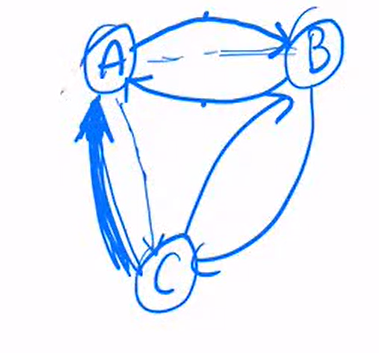
\includegraphics[scale=0.5]{Monte Carlo/images/lect2/img1}\end{center}
We can say, even just by eye inspection that DB is not satisfied.\\
Indeed, the rates from A to B and from B to A are identical, so in principle if detailed balance is satisfied, the probability of seeing the system in A is the same of seeing the system in B.\\
The rates from B to C and from C to B are also identical, and in order for DB to be satisfied, also the probabilities of seeing the system in C and B should be the same.\\
Then if we apply the same argument to C and A, this cannot work anymore: the rate of going from C to A is larger than going from A to C, so in principle the stationary probability of being in A is larger, but this would contradict what we have assumed so far.\\
Therefore $P(A)$ must be different than $P(C)$ and intuitively we could say that $P(A)>P(B)$, and $P(B)>P(C)$, but the explicit calculations should be performed to be sure.\\
In this case there is a \textbf{residual current}, even on the states connected by identical rates.
\smallskip
\\
\textbf{Example 3:}
\begin{center}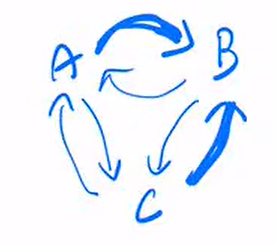
\includegraphics[scale=0.5]{Monte Carlo/images/lect2/img2}\end{center}
Detailed balance should be satisfied in this case. If we assume DB, then clearly $P(A)=P(C)$, and if we also assume that $P(B)>P(A)=P(C)$, because the rate towards B is much bigger than the opposite one, then DB is clearly satisfied.
\smallskip
\\
\textbf{Example 4: }we could think that detailed balance is satisfied because the graph is symmetric, but let's look at the following example to see why this is not necessarily true.\\
\begin{center}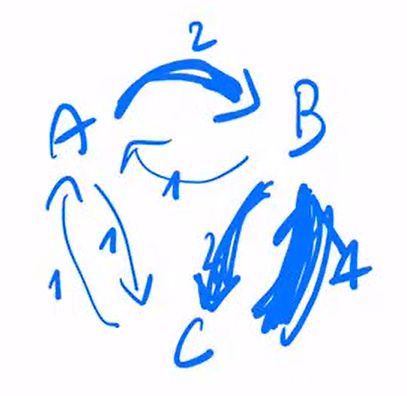
\includegraphics[scale=0.5]{Monte Carlo/images/lect2/img3}\end{center}
In this case detailed balance is satisfied even if the graph is not really symmetric: $P(A)=P(C)=1$, then $P(B) = 2$, because
\[
P(B)=\frac{P(A)\Pi_{A,B}}{\Pi_{B,A}} = \frac{2}{1}=2
\]
for the same argument,
\[
P(B)=\frac{P(C)\Pi_{C,B}}{\Pi_{B,C}} = \frac{4}{2}=2
\]
Then if you have more than one path to reach a specific node, to make sure that detailed balance is satisfied, you should try to reach the same node through different paths and see if you obtain the same results.\\
If this happens, detailed balance is satisfied, otherwise it is not.\\
\subsection{Detailed balance and '1-dimensional' systems}\
\begin{center}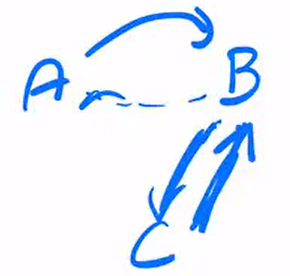
\includegraphics[scale=0.5]{Monte Carlo/images/lect2/img4}\end{center}
In the image above, detailed balance is satisfied (independently from the rates), because if I assign, for example $P(A)=1$, then $P(B)$ can be computed by dividing the rates in the previously shown way.\\
We can repeat the same argument for B and C and then $P(C)$: there is no way to violate DB.\\
Whenever a set of nodes is arranged so that if you pick any pair of nodes, there exists only one path connecting these two, then DB is always satisfied.\\
This is the same thing that happens for a two-state system, where detailed balance and balance are equivalent.\\
\begin{center}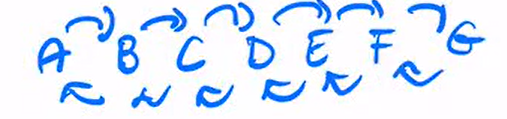
\includegraphics[scale=0.5]{Monte Carlo/images/lect2/img5}\end{center}
For "1-dimensional systems" (systems of any number of nodes where there are many states arranged in a straight line and there is no way to make jumps between states), detailed balance will be satisfied.\\
I cannot find any inconsistencies because there is only one path for going from A to D.\\
For example, as soon as I add, another connection, from G to A, then this is no longer guaranteed: it could either be satisfied or not.
\subsection{Metropolis algorithm}\label{Metropolis}
Let's go back to the algorithm which should sample the surface of a river. We will propose a move and we will either accept it or reject it whether you are on top of the water or not.
We would like to generalize this in order to sample a distribution which is not just constant on the water and 0 elsewhere, but with a preassigned functional form.\\
We preassign $P(x)$, the stationary probability of each state, which for instance could be the canonical distribution.\\
Then I want to be able to generate a Markov chain that draws samples from this distribution and I want to: propose a move $\rightarrow$ decide whether to accept it or not.\\
Balance and detailed balance depend on the presence of a transition matrix $\Pi$, now we are being more specific and we imagine that the transition matrix has a precise form.
We define $M_{x\rightarrow x'}$ as the probability of \textbf{proposing} a move from $x$ to $x'$, and $\alpha_{x\rightarrow x'}$ as the probability of accepting that move, then we have:
\[
\Pi_{x\rightarrow x'} = M_{x\rightarrow x'}\alpha_{x\rightarrow x'}
\]
$M$ is usually defined as \textbf{proposal matrix} or trial matrix: it defines our trial move. In the example of moving on the river where you can move only north and south, it will be a uniform distribution between -1 and 1 that tells you the north-south displacement.\\
We would like to enforce a given $P(x)$\footnote{we are using sometimes $P$ as a function of $x$ and sometimes $x$ as a subscript, it's more intuitive to write it as $P_x$ for discrete systems, but it's the same thing.}, so we want to generate moves in any random way, but we filter on our $P(x)$, based on our acceptance $\alpha$.\\
We will not enforce balance or detailed balance on $M$ or $\alpha$: we will enforce it on $\Pi$.\\
\textbf{Idea for the algorithm:} we want that the position at the next iteration will be either identical to the previous one or the proposed one, the choice is then between two states.\\
Enforcing balance or detailed balance is the same if we limit ourselves in choosing two states, because this is a two-state system \textbf{inside each of the moves}.\\
%If for example we have a system with three states, and we are in state A, we will either propose a move to B or C, after the proposal I apply detailed balance on the subsystem where I only have A and B if B is chosen.\\
$M$ could be any arbitrary matrix, but it should still be a stochastic matrix, without any special symmetry or balance.\\
Then we can enforce DB:
\[
P_xM_{x\rightarrow x'}\alpha_{x\rightarrow x'}=P_{x'}M_{x'\rightarrow x}\alpha_{x'\rightarrow x}
\]
I am assuming that $P$ is assigned, and it will depend on the potential energy function that you want to sample.\\
I fix $M$ and then I want to find how I should accept or reject the moves: $\alpha$.
Then: \[
\frac{\alpha_{x\rightarrow x'}}{\alpha_{x' \rightarrow x}} = \frac{P_{x'}M_{x'\rightarrow x}}{P_xM_{x\rightarrow x'}}
\]
We have to choose two numbers for the acceptance probabilities and I only have a constraint for the ratios of these two values $\rightarrow$ I have an infinite number of choices, but $\alpha$ is a probability, so it must be a number between 0 and 1.\\
I want to accept the moves as frequently as possible, because whenever I reject a move I am wasting an iteration.\\
The best choice is to choose two numbers such that the biggest of the two is 1 and the second one is given by the previously defined ratio:
\[
\alpha_{x\rightarrow x'} = \min\left(1, \frac{P_{x'}M_{x'\rightarrow x}}{P_xM_{x\rightarrow x'}}\right)
\]
\begin{equation*}
    \alpha_{x'\rightarrow x} =\frac{1}{\max\left(1, \frac{P_{x'}M_{x'\rightarrow x}}{P_xM_{x\rightarrow x'}}\right)}
\end{equation*}
This way of operating is called \textbf{Metropolis rule}.
Basically, we compute the ratio and, if it is larger than one, I assign to $\alpha_{x\rightarrow x'}$ the value of 1. Then, if this is true, the ratio for the opposite transition will be smaller than 1, since they are reciprocal.\\
\noindent\rule{8cm}{0.4pt}\\
\textbf{Digression: Symmetric rule}\\
This is not the only possible choice, there is another one which is also sometimes used, which is the \textbf{symmetric rule}.
\[
\alpha_{x\rightarrow x'} = \frac{P_{x'}M_{x'\rightarrow x}}{P_{x'}M_{x'\rightarrow x}+P_xM_{x\rightarrow x'}}
\]
We can see that this also works because if we swap $x$ with $x'$, the denominator is going to be the same one, then the ratio between the acceptance probabilities will be the correct one.\\
\noindent\rule{8cm}{0.4pt}\\
What could be seen though is that Metropolis rule will be the one which will give the highest possible acceptance.\\
\subsubsection{Metropolis algorithm: example}
Let's see how to implement it with a pseudocode:\\
\begin{minipage}{\textwidth}
\renewcommand*\footnoterule{}
\begin{savenotes}
\begin{algorithm}[H]\label{metropolis_generic}
			\caption{Monte Carlo with Metropolis rule}
			\begin{algorithmic}[0]
				\State p0=p(x)
				\For{istep in range(nsteps)\footnote{My iterations are no longer going to be on time steps, but are just iterations over my Markov Chains. Sometimes \texttt{nsteps} is referred to as \textit{Monte Carlo time}}}
					\State xtry = trial(x)\footnote{This function only takes the value of $x$, the current position, as an argument: no other info about the history of the system. It gives a new attempt position.}
					\State ptry = p(xtry)\footnote{Probability in the trial position, this will be the expensive calculation, because generally computing the energy of the state is the most expensive operation.}
					\State alpha =  $\frac{ptry}{p0}$\footnote{I only need the ratio between these probabilities. If we compute in terms of energy, this will be $\mathbf{e^{-\beta(U(xtry)-U(x))}}$. In principle this probability should contain the partition function, but here the normalization does not enter, since we are computing the ratio. I don't need to know the partition function and this is a good thing, because computing partition functions is usually quite expensive.}$\frac{M_{xtry \rightarrow x}}{M_{x\rightarrow xtry}}\footnote{This term is often NOT included, because when the probability of proposing a move and the opposite one are identical, they cancel each other. If they are not identical, this term must be included or we would make a mistake.}$
					\If{alpha $>$ 1\footnote{\textbf{This coincides with Metropolis rule}, when we take the minimum between 1 and the ratio. We could in principle set it to any number bigger or equal than one, and then avoid this step, but if we want to quantify the average acceptance, this step is necessary.}}
						\State alpha = 1
					\EndIf
					\If{alpha $>$ rand()\footnote{I accept the move or reject the move with $\alpha$ probability.}}
						\State x = xtry
						\State p0=ptry
					\EndIf
				\EndFor
			\end{algorithmic}
		\end{algorithm}
\end{savenotes}
\end{minipage}
\textbf{Examples for $M$:}
If we consider a three-state system, if I'm in state 1 I can propose to go to states 2 or 3 with the same probability.\\
Then when I'm in 2 I'm going to propose to go to 1 or 3, again with the same probability.\\
Then the proposal matrix would be symmetric and the ratio between the proposals could be disregarded.\\
If I propose my moves in such a way that the probability of proposing the backward and the forward moves is not identical, then it is not a problem, but this should be taken into account in the acceptance.\\
\noindent\rule{8cm}{0.4pt}\\
\textbf{Digression: }sometimes there are very good reasons for the proposal matrix not to be symmetric.\\
Sometimes people try to design smarter moves in order to have a higher acceptance.\\ 
If the transition matrix is symmetric, the acceptance will be always 1 when the new energy is lower than the previous one, because $e^{-\beta(U(xtry)-U(x))}$ will be bigger than 1.\\ 
Then a conformation with a lower energy will \textbf{always} be accepted.\\
Let's say that there is a force acting on the system, we compute it and we favour the proposal of moves in the direction corresponding to the force. It is very likely that the energy will decrease, the acceptance will be high and Monte Carlo would be very efficient, but we \textbf{must} not forget the ratio between the terms of the proposal matrix.\\
\noindent\rule{8cm}{0.4pt}\\
If we think of a molecular system, we could operate in the following way: we pick a random atom, and then we pick a random direction between $(x,y,z)$. We then choose a random displacement and we take the new conformation, compute the energy and decide whether to accept or reject the moves. This algorithm would have a symmetric $M$.\\\\
The previous algorithm only computes a Markov chain.\\
Let's say that now we want to compute the average value of a function.\\
\begin{minipage}{\textwidth}
\renewcommand*\footnoterule{}
\begin{savenotes}
\begin{algorithm}[H]\label{metropolis_with_average}
			\caption{Average estimation}
			\begin{algorithmic}[0]
				\State p0=p(x)
				\State \underline{\emph{sum = 0}}
				\For{istep in range(nsteps)}
					\State xtry = trial(x)
					\State ptry = p(xtry)
					\State alpha =  $\frac{ptry}{p0}\frac{M_{xtry \rightarrow x}}{M_{x\rightarrow xtry}}$
					\If{alpha $>$ 1}
						\State alpha = 1
					\EndIf
					\If{alpha $>$ rand()}
						\State x = xtry
						\State p0=ptry
					\EndIf
					\State \underline{\emph{sum += f(x)}\footnote{\texttt{f} could be the depth of the river, or any observable that depends on the coordinates of your system.}}
				\EndFor
			\end{algorithmic}
		\end{algorithm}
\end{savenotes}
\end{minipage}
We can see that rejecting a move means accepting a move where the system goes in the same place it was at the previous step.\\
\\\begin{comment}
\textbf{Q1: }To compute the average, shouldn't we sum over samples which are distant in the Markov-Chain at least something comparable to the autocorrelation time of the Markov Chain?\\
\textbf{A1: }Not necessarily, these samples are drawn from a distribution that is guaranteed to be the one defined in $P(xtry)$. These samples are not independent and it's not necessary to have independent samples.\\
\end{comment}
\noindent\rule{8cm}{0.4pt}\\
\textbf{Autocorrelation time considerations:}\\
\textbf{Q: }To compute the average as the sum, shouldn't all samples be independent?\\
\textbf{A: }That is not true. What you are saying is true to estimate the error, not the mean or the variance. The mean and the variance can be computed even with non-independent samples.\\ 
\textbf{Example: }We can generate 10 independent samples, then take take each of these samples twice. We will have a trajectory made of 20 points, pairwise a repetition of the previous 10, so they are clearly not independent.\\
The average is going to be identical and it's not going to be worse than the previous one. If we think though that the error is related to the standard deviation, divided by the number of points, then this will not hold.\\
This will hold only if the 20 points are all independent.\\
\noindent\rule{8cm}{0.4pt}\\
There are two ingredients in this algorithm:
\begin{itemize}
\item move proposal and computation of an acceptance rate depending on the distribution we want to sample;
\item Metropolis rule, the $\min$ function to compute the acceptance
\end{itemize}
The expensive part is the computation of the energy of the new conformation, so we would prefer to accept as many moves as possible, in order to arrive more quickly to a conformation that is independent from the current one.\\
The speed at which the statistical error will decrease depends on how independent conformations are from each other.\\
Clearly then we want our moves to be as 'big' as possible, so that the proposed arrival state should be as different as possible from the previous state, but not so different that you don't exploit anymore the fact that states with a reasonable probability are close to each other.\\
To understand this concept, we can think again on the example of the river: the bigger the step size, the lowest the acceptance will be, because a big step size draws you away from the river.\\
\subsection{Trial($x$) definition, $\Delta$ considerations}
We must then define the function trial(x):\\
\begin{algorithm}[H]\label{trial}
			\caption{Trial function}
			\begin{algorithmic}[0]
				\Function{trial}{$x$}
					\State return x + $\Delta$*(rand()*2-1)
				\EndFunction
			\end{algorithmic}
		\end{algorithm}
Basically \texttt{rand()*2-1} will be a random number between -1 and +1, and $\Delta$ will define the maximum jump I will be able to do. $\Delta$ will be in the same units of $x$.\\
$\Delta$ is called step size and tells us how different the next set of coordinates will be  from the previous one.\\
There is some analogy between $\Delta$ and the time step in molecular dynamics simulations.\\
If the time step is very small in MD, you will have very accurate trajectories, but the system will take a very long time to evolve: the same thing holds for $\Delta$.\\
The difference will be when these two parameters are large: in MD simulations, when the time step becomes too big, you start to obtain incorrect results.\\
\textbf{If $\mathbf{\Delta}$ is too large, the acceptance drops down}.\\
Monte Carlo is a way to propose moves randomly and then correct them a posteriori, by discarding the incorrect moves, thanks to the acceptance. This guarantees that you will always obtain correct results.\\ 
If the acceptance is basically 0, the samples will all be identical and the algorithm is, in practice, not ergodic.\\
\subsubsection{Optimal choice for $\Delta$}
The optimal choice for $\Delta$ will depend on the scale of your system. Similarly to the time step, also here the 'stiffness' of the potential energy will determine the optimal size of $\Delta$.\\
A bigger $\Delta$ can be used if there are soft interactions, a smaller one when they are stiff. \textbf{The optimal value of $\Delta$ is system-dependent}.\\
The proper way to optimize the choice of this parameter, we should try to run the simulation with a certain $\Delta$, then compute the autocorrelation time of the system, change $\Delta$ and find the \textbf{value which minimizes the autocorrelation time.}\footnote{\textit{Bussi suggests to have a look at Block Analysis, he has actually never defined the autocorrelation time. Not defined by Bussi, but just to give an idea: \emph{autocorrelation represents the degree of similarity between a given time series and a lagged version of itself over successive time intervals.}}}\\
Formally, what we could also do, once we define the matrix $\Pi$, is to compute its eigenvalues and eigenvectors. We want the second eigenvalue(the first is 1) to be as small as possible.\\
This would tell that any information about the current state of the system will be lost on a timescale which is related to the size of that eigenvalue.\\
Anyway, this can be done only in cases when you can manipulate things analytically.\\
What is typically done is to compute the average of an observable and its autocorrelation time, then the best answer will depend on the chosen observable.\\
The optimal $\Delta$ will then vary depending on the observable over which we are minimizing the autocorrelation time.\\
In general, the potential energy is the observable which is used as a metric.\\
Sometimes, \textbf{mistakenly} the optimal $\Delta$ is defined as the one which gives the average acceptance equal to $\frac{1}{2}$. Indeed if it were 0 the autocorrelation time of any observable would be infinite. If it were 1 all the moves would be accepted: this (generally) happens if $\Delta$ = 0.\\
Therefore the (wrong) argument would be that the optimal value should be $\frac{1}{2}$. This is although \textbf{not correct}.\\
The right way to optimize $\Delta$ is to: \textbf{compute the statistical error of a quantity} you are interested in and \textbf{minimize it}.
\subsubsection{Algorithm example for moving more than one atom}
\textbf{Example: }Let's say that I have 10 atoms and I want to move them. When I apply Monte Carlo I should choose which atom to move, and there are two possible ways to do it:
\begin{itemize}
\item \textbf{randomly}: I pick randomly one of the atoms at each step;
\item \textbf{sweep}: I first move atom number 0, then 1 and so on.
\end{itemize}
Let's see how sweep is implemented.\\
\begin{minipage}{\textwidth}
\renewcommand*\footnoterule{}
\begin{savenotes}
\begin{algorithm}[H]\label{sweep}
			\caption{Sweep}
			\begin{algorithmic}[0]
				\For{istep in range(nsteps)}
					\For{iatom in range(natoms)}
						\State xtry=x.copy()\footnote{.copy() is added otherwise you would get a copy reference, just a technical note from Bussi.}
						\State xtry[iatom] = trial(x[iatom])
						\State [...]
						\State [Metropolis]
						\State [...]
					\EndFor
				\EndFor
				
			\end{algorithmic}
		\end{algorithm}
\end{savenotes}
\end{minipage}
Will this algorithm satisfy detailed balance? If we consider the forward and backward simulations we can clearly see that detailed balance is not satisfied, because the opposite trajectories are different.\\
The transition matrix basically becomes time-dependent, because Metropolis algorithm will be performed inside an iteration over atoms.
To understand why detailed balance is not satisfied, we could add another variable which describes the index of the atom that I have moved at the last iteration.\\
The moves on the positions are then satisfying detailed balance, but the moves over the indices of the atoms will NOT satisfy DB.\\
How could we modify this algorithm to enforce detailed balance?\\
Choosing the atom randomly would be sub-optimal, because if there are N atoms, after N iterations there will be many atoms which still have not moved, and some others which have moved more than once. It is not very efficient.\\
Before every sweep we should \textbf{choose randomly the direction of the sweep}: half of the time the sweep will be done backwards and half of the time it will be done forward. This will be enough to enforce detailed balance.\\
\noindent\rule{8cm}{0.4pt}\\
\textbf{Q: }What would be something which we can only obtain with an algorithm which enforces DB and not with one which only enforces balance?\\
\textbf{A: }Equivalence between forward and backward trajectories. It is not necessary if we want to get average quantities from a sample, for example. But if you want to compute properties of the trajectory, it may be relevant to enforce DB.\\\begin{comment}
\textbf{Q2: }Could it also affect the autocorrelation time?\\
\textbf{A2: }By construction, the minimum autocorrelation time algorithm ('+' in the figure) is more likely to fall inside the algorithms which enforce balance and not detailed balance.\\
\begin{center}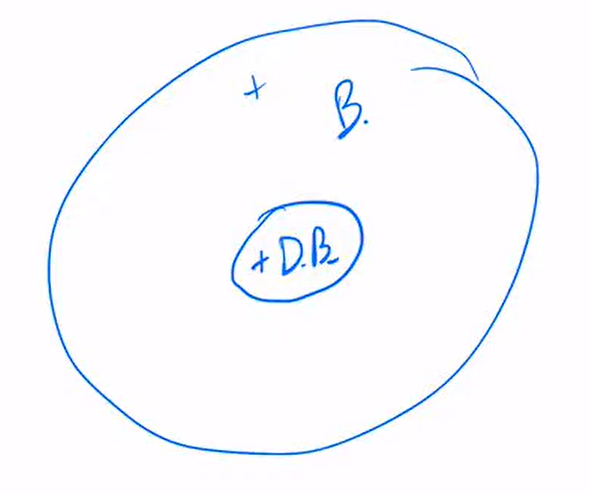
\includegraphics[scale=0.35]{Monte Carlo/images/lect2/img6}\end{center}
This is because clearly DB algorithms are a subset of algorithms which enforce balance, anyway it's not easy to design algorithms which are efficient in terms of minimizing the autocorrelation time.\\ 
Therefore if the purpose of the algorithm is the one of making it efficient, \textbf{do not focus on DB} also consider balance.\\\end{comment}
\noindent\rule{8cm}{0.4pt}\\
\subsection{Generalized detailed balance}
It is something more general than detailed balance, but much more specific than balance.\\
We want to show that Hamilton equations satisfy generalized detailed balance.\\We can show that they do not satisfy detailed balance.\\
\begin{center}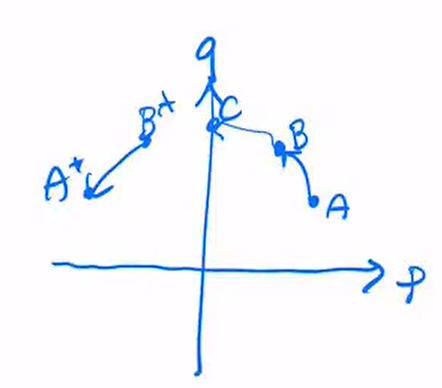
\includegraphics[scale=0.35]{Monte Carlo/images/lect2/img7}\end{center}
I can define a transition matrix $\Pi$, even if it is deterministic, using delta functions.\\
Detailed balance is clearly not satisfied, because given a trajectory, the probability for the backward trajectory is exactly 0.\\
We can use time reversibility and change the sign of the velocities: instead of compensating the transition from A to B with an equally likely transition from B to A, I compensate it with an equally likely transition from B* to A*.\\
B* and A* will be defined in the following way:
\[x = (p, q) \rightarrow x\text{*} = (\mathbf{-p}, q)\]
Formally, we say that $P(x)=P(x\text{*})$, because if we change the sign of the momenta, these only enter in the distribution through the kinetic energy, which is an even function of the momenta.\\
\[P(x)P(x\rightarrow x') = P(x'\text{*})P(x'\text{*}\rightarrow x\text{*})\]
This condition is different than detailed balance, and it also implies balance, one just needs to
sum over all the possible transitions.\\
Let's say now that I use Hamilton equations to sample points in the canonical ensemble: the energy will be constant, clearly the dynamics will have a stationary distribution, but it is non-ergodic.\\
It will be non-ergodic because once a value of the energy is given, only states with the same value of energy will be visited. Since there is a constant of motion, the system cannot be ergodic.\\
One could use Velocity Verlet: energy is not constant, but will detailed balance be satistified?\\
Velocity Verlet preserves the volume in the phase space, and the algorithm is time reversible, then  detailed balance will hold.\\
I could then use velocity Verlet algorithm to generate moves for Monte Carlo, and compute the acceptance just by looking at how much the energy changed. Then we can use Velocity Verlet to generate moves for Monte Carlo.\\
Acceptance equal to one would correspond to exact conservation of the energy.\\
This is the core of the so-called Hybrid Monte Carlo.